\subsubsection{Design}

The $V_{DS}$ fall time (the MOSFET switch-in time) is slowed down to $\approx 250ns$ and the rise time (switch-off) is $\approx 50ns$. The required resistor values can be calculated using Equation \ref{eq:i_Gsink_per_fet_1} through Equation !!!. \\

To get the resistor values, first, the sink current must be calculated to draw the gate charge in the required switch-off time for the individual MOSFETs. 

    \begin{equation}
        i_{Gsink/FET} = \bigg( \frac{Q_{GD}}{t_{sw{\_}off}} \bigg)
        \label{eq:i_Gsink_per_fet_1}
    \end{equation}
    
    where
    
    \begin{itemize}
        \item $i_{Gsink/FET}$ is the required switch-off current
        \item $Q_{GD}$ is the gate-drain charge of the MOSFET
        \item $t_{sw{\_}off}$ is the desired switch-off time
    \end{itemize}
    
    \begin{equation}
        i_{Gsink/FET} = \bigg( \frac{V_{Miller}}{R_{G{\_}FET} + R_{G{\_}FET{\_}int}} \bigg)
        \label{eq:i_Gsink_per_fet_2}
    \end{equation} \\
    
    Rearranging Equation \ref{eq:i_Gsink_per_fet_2} yields the following:
    
    \begin{equation}
        R_{G{\_}FET} = \bigg( \frac{V_{Miller}}{i_{Gsink/FET}} - R_{G{\_}FET{\_}int} \bigg)
        \label{eq:i_Gsink_per_fet_2}
    \end{equation}
    
    where
    
    \begin{itemize}
        \item $R_{G{\_}FET}$ is the resistor for the individual MOSFETs
        \item $V_{Miller}$ is the Miller-plateau of the MOSFET
        \item $R_{G{\_}FET{\_}int}$ is the internal gate-source resistance of the MOSFET
    \end{itemize}
    
    Now the switch-on current and common resistance can be calculated:
    
    Taking after Equation \ref{eq:i_Gsink_per_fet_1}:

    \begin{equation}
        i_{Gsource/FET} = \bigg( \frac{Q_{GD}}{t_{sw{\_}on}} \bigg)
        \label{eq:i_Gsource_per_fet_1}
    \end{equation}    
    
    
    
    \begin{equation}
        i_{Gsource/FET} = \frac{\frac{V_G - V_{Miller}}{R_{pullup} + R_G}}{N}
        \label{eq:i_Gsoursce_per_fet_2}
    \end{equation}
    
    and
    
    \begin{equation}
        R_G = R_{G{\_}common} + \frac{R_{G{\_}FET} + R_{G{\_}FET{\_}int}}{N}
        \label{eq:R_G}
    \end{equation}
    
    Substituting Equation \ref{eq:R_G} into Equation \ref{eq:i_Gsoursce_per_fet_2} and rearranging them yields the following:
    
    \begin{equation}
        R_{G{\_}common} = \frac{i_{Gsource/FET} \cdot N}{V_G - V_{Miller}} - R_{pullup} - \frac{R_{G{\_}FET} + R_{G{\_}FET{\_}int}}{N}
        \label{eq:R_G_common}
    \end{equation}
    
    It is easy to see that when $N = 2$, the total current to be supplied and drawn by the driver is double of the indivdual MOSFETs.
    
    
    \begin{equation}
        i_{Gsource{\_}total} = i_{Gsource/FET} \cdot 2
        \label{eq:i_G_source_total}
    \end{equation}
    
    \begin{equation}
        i_{Gsink{\_}total} = i_{Gsink/FET} \cdot 2
        \label{eq:i_G_sink_total}
    \end{equation}
    
    The following variables and their values, obtained from their respective datasheets or calculated, were used:
    
    \begin{itemize}
        \item $i_{Gsource/FET} = 136 mA$ is the required switch-on current per MOSFET
        \item $i_{Gsource{\_}total} = 272 mA$ is the required total switch-on current
        \item $i_{Gsink/FET} = 680 mA$ is the required switch-off current per MOSFET
        \item $i_{Gsink{\_}total} = 1.36 A$ is the required total switch-off current
        \item $Q_{GD} = 34 nC$ is the gate-drain charge of the MOSFET
        \item $t_{sw{\_}on} = 250 ns$ is the desired switch-on time
        \item $V_G = 12V$ is the gate voltage applied
        \item $V_{Miller} = 4.4 V$ is the Miller-plateau of the MOSFET
        \item $R_{pullup} = 2.6 \ohm$ is the gate driver IC internal pullup resistance
        \item $R_G = 25.34 \ohm$ is the equivalent resistance seen by the gate driver
        \item $R_{G{\_}common} = 22.1 \ohm$ is the common resistance value
        \item $R_{G{\_}FET} = 5.17$ is the resistor for the individual MOSFETs
        \item $R_{G{\_}FET{\_}int} = 1.7 \ohm$ is the internal gate-source resistance of the MOSFET
        \item $N = 2$ is the number of parallel MOSFETs
    \end{itemize}
    
    The diode parallel to the common resistor introduces a forward voltage drop of up to $900 mV$ when draining the gate of charge. It should not cause problems, since as Figure \ref{fig:mosfet_transfer_char} shows, the drain current of the MOSFET is insignificant in that region.
    
\begin{figure}[H]
	\centering
	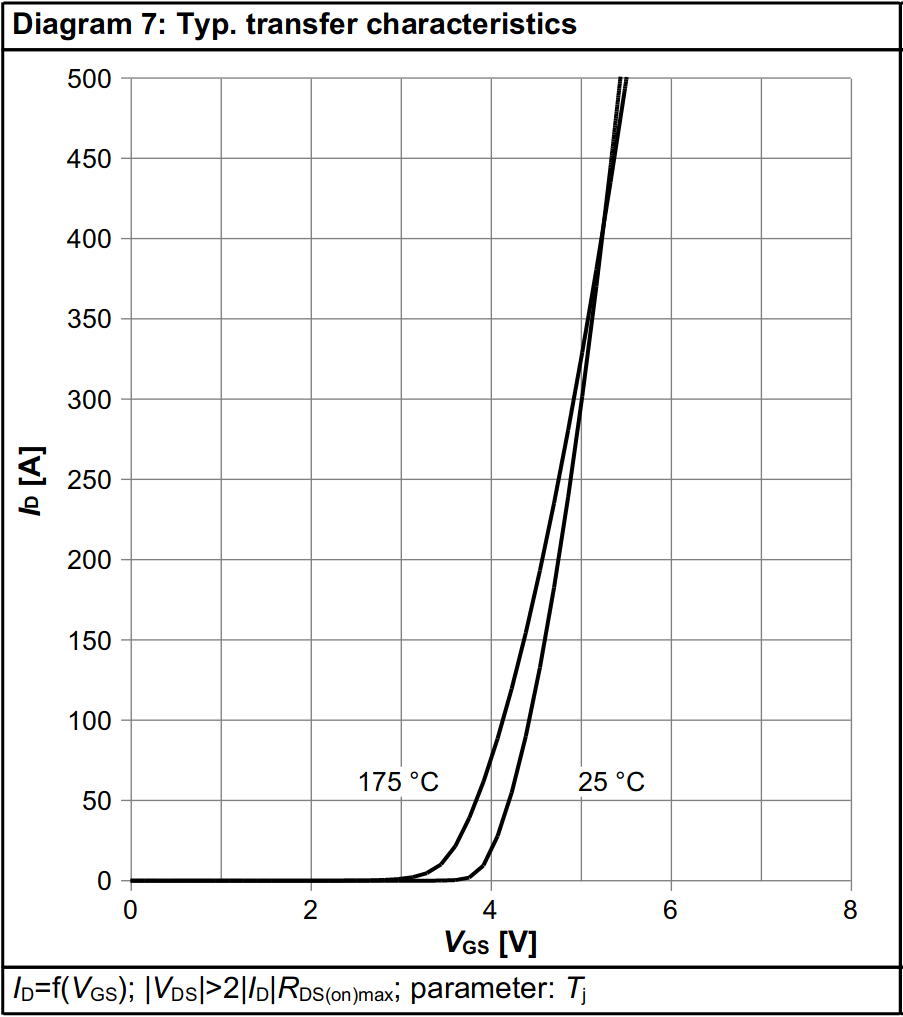
\includegraphics[width=0.6\linewidth]{pictures/hardware/Driver_Board/mosfet_transfer_char.png}
	\caption{Typical transfer characteristics of a MOSFET}
	\label{fig:mosfet_transfer_char}
\end{figure}